%SIGMETRICS
\documentclass{sig-alternate}

%USENIX
%\documentclass[letterpaper,twocolumn,10pt]{article}
%\usepackage{usenix,epsfig,endnotes}
\usepackage{amsmath}
\usepackage[noend]{algpseudocode}
\usepackage{paralist,algorithm}
\usepackage{booktabs}
\usepackage{subcaption}
\usepackage{multirow}
\usepackage{float}
\usepackage{graphicx}
\usepackage{pgfplots}
\usepackage{amssymb}
\usepackage{epstopdf}
\usepackage{tikz}
\usepackage{tkz-tab}
%\usepackage{titlesec}
\usepackage{xspace}
%\usepackage{epsfig}
%\epstopdfsetup{outdir=./}
%\usepackage[showframe=true]{geometry}
\usepackage{enumitem}
\usepackage{adjustbox}
\usepackage{verbatimbox}

\begin{document}

\title{Budget Limited Adaptive Live Debugging}

\iffalse
\author{
{Nipun Arora$^\dagger$, Franjo Ivan\v{c}i\'{c}}\\$^*$, Gail Kaiser$^\ddagger$}\\
$^\dagger$NEC Laboratories America \hspace{1.4cm}   $^\*$Google NYC \hspace{1.4cm}  $^\ddagger$Columbia University\\
nipun@nec-labs.com \hspace{4pt} ivancic@google.com \hspace{4pt} kaiser@cs.columbia.edu \\
}
\fi

%\iffalse
\author{
{Nipun Arora}\\
       NEC Labs\\
%       Princeton, NJ, USA\\
       nipun@nec-labs.com
\and
{Franjo Ivan\v{c}i\'{c}}\\
       Google NYC\\
%       New York, NY, USA\\
       ivancic@google.com
\and
{Gail Kaiser}\\
       Columbia University\\
%       New York, NY, USA\\
       kaiser@cs.columbia.edu
}
%\fi
\maketitle


\newcommand{\iprobe}{\texttt{iProbe}\xspace}
\newcommand{\livedebugging}{\emph{Live Debugging}\xspace}
\newcommand{\parikshan}{\texttt{Parikshan}\xspace}
%\newcommand{\comment}[1]{}
\newtheorem{example}{Example}
\def\infinity{\rotatebox{90}{8}}


\begin{abstract}
  
%Existing Testing and Verification technologies, are impractical for testing large scale softwares. 
%One of the biggest problems faced by developers debugging large scale systems is replicating the deployed environment to figure out errors.
%Additionally, most modern companies are combining their development and operation management activities (DevOps), which has led to an increased emphasis on fast bug resolution.
%In recent years there has been a lot of work in record-and-replay systems which captures traces from live production systems, and replays them.
%However, most such record-replay systems have a high recording overhead and are still not practical to be used in production environments without paying a penalty in terms of user-experience. 
In this work we present a framework which allows users to debug a target production system (execution tracing, profile, breakpoint etc.) in a sandbox environment cloned from the live running system at any point in its execution.
% of a service oriented application. 
The paper leverages user-space containers (OpenVZ/LXC) to launch a container cloned and migrated from running instances of an application, thereby launching two containers: production (which provides the real output), and debug-container (for debugging). 
This \emph{debug-container} provides a sandbox environment for safe application of instrumentation tools without any perturbation to the actual production environment. 
%Test cases are initiated using user-defined probe points which launch test-cases using the execution context of the probe point. 
%Our sandboxes provide name-space, and resource management for the processes executing the test/debug cases.
A customized-network proxy agent replicates inputs from clients to both the production and debug-container, as well as safely discards all outputs from the debug-container.
%These sandboxed test-containers can be run either on the same physical host as the production container, or scaled out on dedicated physical test servers.
%, and manage the file system such that existing and newly created file descriptors are safely managed.
%Further we explain fidelity guarantees of our proposed system
We believe our tool provides a novel mechanism for practical live-debugging of large scale multi-tier and cloud applications, without requiring any application down-time, and minimal performance impact.
%In our evaluation provide a number of use-cases to show the utility of our tool.  
\end{abstract}

\section{Introduction}
\label{sec:intro}

\begin{figure*}[ht!]
	\begin{center}
		%    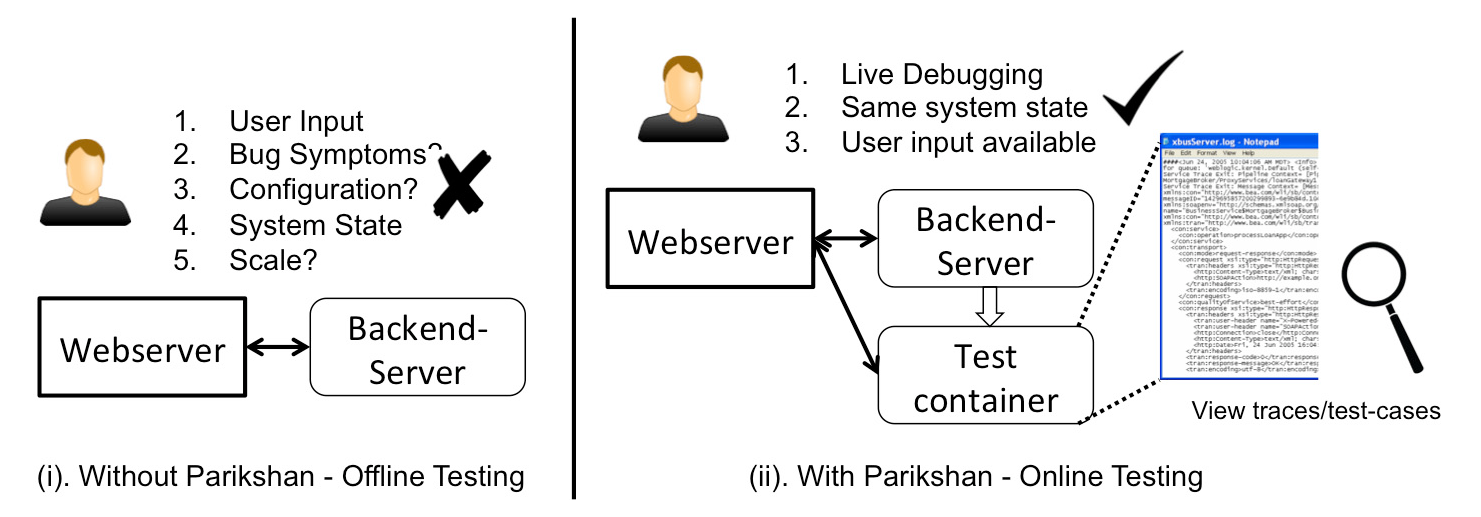
\includegraphics[width=0.7\textwidth]{figs/motivation.eps}
		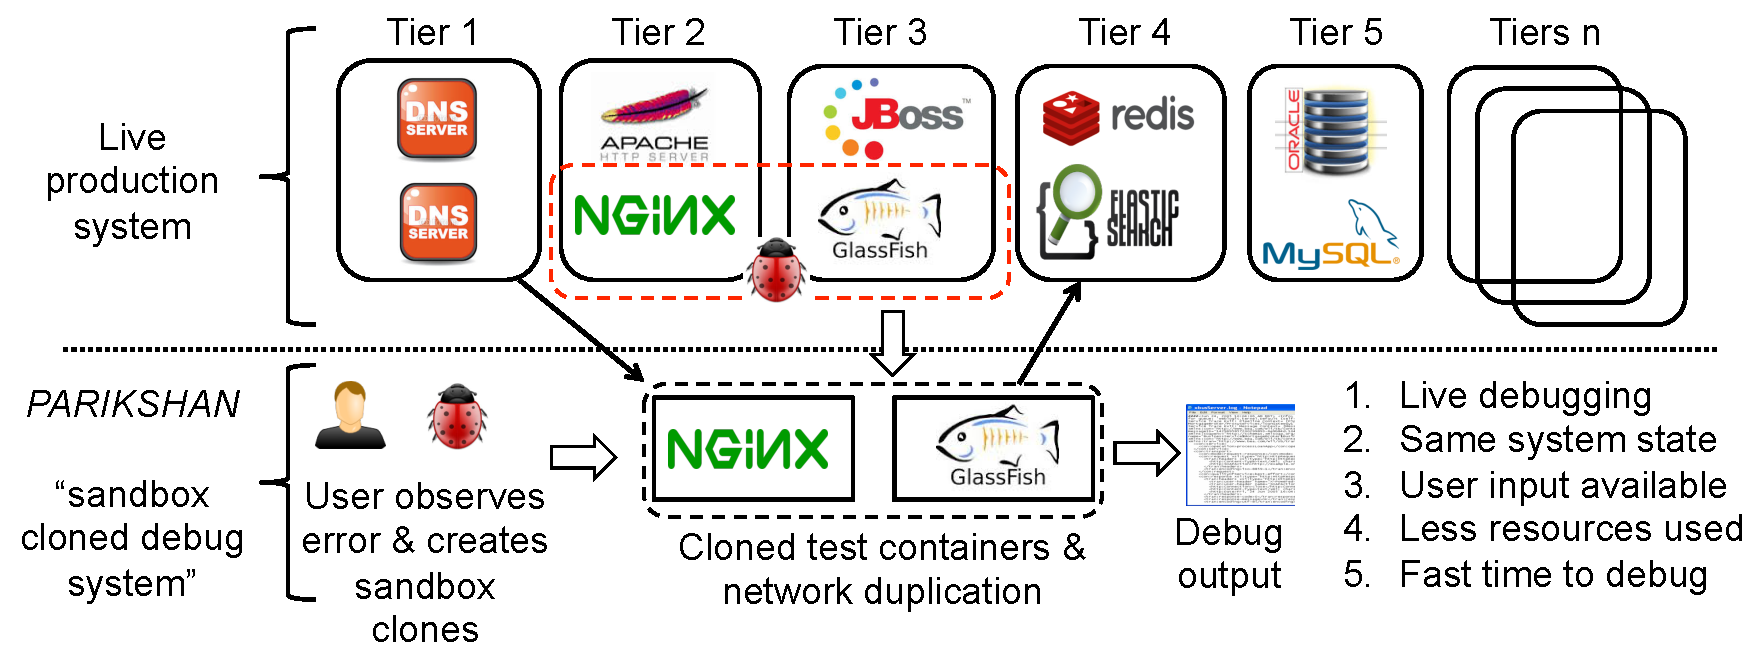
\includegraphics[width=0.9\textwidth]{figs/workflow3.pdf}
		\caption{Workflow of \parikshan in a live multi-tier production system with several interacting services. When the administrator of the system observes errors in two of it's tiers, he can create a sandboxed clone of these tiers and observe/debug them in a sandbox environment without impacting the production system.}
		\label{fig:motivation}
	\end{center}
\end{figure*}

Rapid resolution of incidence~(error/alert) management~\cite{sasase2013} in online service oriented systems is extremely important.
However, the complexities of virtualized environments coupled with large distributed systems have made bug localization harder. 
%The large scale of such systems means that any downtime has significant financial penalties for all parties involved.
On the other hand, there is a trend in the software engineering industry towards closer coupling between software developers and operators~(DevOps~\cite{devops}) in order to have shorter release and debug cycles 
(Facebook mobile has 2 releases a day, and Flickr has 10 deployment cycles per day~\cite{10DevOps}). 
%This re-emphasizes the need to have a very short time to diagnose and fix a bug.
Hence, debugging is hard not only because of difficulty to capture the root-cause, there is also an increased emphasis on the need to localize and fix bugs in a short period of time.

%Furthermore, whether to repair flaws or add features, software patches are released all the time.
%For instance, Facebook mobile has 2 releases a day, and Flickr has 10 deployment cycles per day~\cite{10DevOps}).
%Hence, it is increasingly important to localize and fix bugs in a very short period of time.
%As application software grows and gets more complicated, debugging large scale applications has become increasingly important. 
%This problem is further compounded by the recent trend in software engineering industry by large companies towards DevOps \cite{devops}. 
%The recent trend towards DevOps~\cite{devops} by the software engineering industry further compounds this problem. 
%by requiring a fast and rapid resolution towards any software bug.
%DevOps stresses on close coupling between software developers and operators, in order to have shorter release cycles (Facebook mobile has 2 releases a day, and Flickr has 10 deployment cycles per day~\cite{10DevOps}). 
%This re-emphasizes the need to have a very short time to diagnose and fix a bug.
%Hence, debugging is hard not only because of difficulty to capture the root-cause, it is also increasingly important to localize and fix bugs in a very short period of time.

Existing state-of-art techniques for monitoring production systems~\cite{dtrace, iProbe, winetw} rely on light-weight dynamic instrumentation to capture execution traces. 
Operators then feed these traces to analytic tools~\cite{magpie,clue} or do offline debugging, to find the root-cause of the error.
However, dynamic instrumentation has a trade-off between granularity of tracing and the performance overhead. 
Operators keep instrumentation granularity low, to avoid higher overheads in the production environment.
This often leads to multiple iterations between the debugger and the operator, to increase instrumentation in specific modules, in order to diagnose the root-cause of the bug. 
%To avoid higher overheads instrumentation granularity is generally kept low, thereby making bug diagnosis harder.
%Debugging is a lengthy process: debuggers try to piece together what could be the possible problem using log information.
%Often more information is required to understand the context better which leads to several iterations before the problem is debugged, thereby increasing the time-to-debug.

Another body of work has looked into record-and-replay~\cite{odr,revirt,laadan2010transparent,geels2007friday} systems which capture execution traces, in order to faithfully replay them in an offline environment.
These systems try to capture system level information, user-input, as well as all possible sources of non-determinism, to allow for in-depth \textit{post-facto} analysis of the error.
%Another tool, aftersight~\cite{aftersight} looks into recording, and replaying the execution in parallel, to allow for decoupled analysis. 
However, owing to the amount of instrumentation required, record-and-replay tools introduce an even heavier overhead. 
This may make them unacceptable for several user-facing systems where performance is essential.


%However, it is extremely difficult to meet the quick debugging demands of a devops environment, as it is not feasible to recreate realistic workloads in an offline development environment for large scale multi-tier or cloud based applications.
%\noindent
%Existing techniques for monitoring production systems~\cite{dtrace, iProbe, winetw} rely on light-weight dynamic instrumentation in either the kernel or the application. 
% kernel, application or error logs.  
%as a mechanism to localize and identify the bugs as well.
%There are several problems with these techniques:
%\begin{itemize}[leftmargin=*,topsep=0pt,itemsep=-1ex,partopsep=1ex,parsep=1ex]
%\textbf{Unrealistic} because 
%\item %These techniques rely on instrumentation to gather execution traces.
%Dynamic instrumentation has a trade-off between granularity of tracing and the performance overhead. 
%Operators usually avoid high instrumentation in live production system.
%Hence, the logs captured may not be enough to find root-cause of the error.
%\item Applications use a variety of third party plugins, are deployed on multiple kernels, which makes generating configurations and state of production systems difficult. 
 % traditional whitebox testing in the development environment is unable to capture these bugs.
%\item Debugging is a lengthy process: Developers try to piece together what could be the possible problem using log information.
%Often more information is required to understand the context better which leads to several iterations before the problem is debugged.
%\end{itemize}

%\noindent
%Recent work in record-and-replay~\cite{} tools allows operators to capture the context of the application and reproduce bugs in an offline environment.
%However, these tools incur a relatively high overhead, and can thereby not be used in production systems. 

%One of the proposed mechanisms of addressing this problem is to ``perpetually test''~\cite{perpetual} the application in the field after it has been deployed. 
%This is important since testing in a production system enables us to capture previously ``unreachable'' system states, which can arise due to various factors such as unpredictable user environment, outdated software, an ever increasing list of hardware devices (e.g. mobile phones, embedded devices etc.), or simply because of imperfect network connectivity (wifi, cellular).
%which are possible only for a long running production environment. 
%Since we are testing in a real environment, we get real user-input for test-cases, and are able to test a real environment.
%However, perpetual testing has never gotten much traction because of an obvious flaw : executing such test-cases will adversely effect the user-experience, both in performance and potentially in application logic.

%\noindent
%Previous approaches such as Chaos Monkey~\cite{chaosmonkey} from Netflix and AB Testing~\cite{abtesting} already use ``testing in the wild'' to check for errors and robustness of the software or to check for new features that have been added.  
%However, despite a clear need, debugging in the production environment has never gotten much traction in real-world applications as it may consume too much performance bandwidth and more importantly, it can impact the sanity\footnote{The state of the production server may change leading to a crash or wrong output} of real operational state of the software.
%Another trend embraced by mainstream companies such as Flickr, Twitter, Facebook and Google is DevOps\cite{devops}. 
%And wile testing, analyzing and monitoring are an important aspect of the devops cycle, usually only a very small performance bandwidth in the production server can be dedicated to QA operations as compared to real user activity(so as to not effect user-perceived delay). 

%Embedding test-case logic within the context of the application will result in state-change, or performance slow-down that would otherwise not be there in an optimized implmentation of the application.
%This is something which is usually unacceptable in user-facing applications.
%The authors have previously looked into amortizing the cost of running the test, by running it in parallel \cite{invite}.
%However such approaches cannot completely avoid the slowdown, and additonally do not completely sandbox the effects of the test case on the production server. 

%An alternate approach is to record live applications, and replay them offline.
%Over the years there have been several systems which have explored this direction with promising results.
%However most record and replay systems have high overheads, and require replication of the running configuration which may not be possible. 
%Additionally the administrator needs to wait for offline analysis, instead of doing real-time diagnosis.

%On the other hand, there has been an impressive increase in the scale of computing resources, and distributed scalability of infrastructure.
%Web based applications are often hosted in cloud environments, this allows for easily scaling up the hardware resources.
%This often allows for redundant computation, which can be used for testing purposes. 

%The main reason that debugging in the development environment is easier, is because developers can trace the execution flow of the program using tools such as gdb~\cite{gdb}, valgrind~\cite{valgrind} etc. and look at variable values for the given input. 
%This gives them an immediate insight as to whether the application is behaving correctly, and where the bug could be.
%Unfortunately, such techniques are not possible in the production environment as they would lead to unacceptable slow-down, alter the application functionality, or worse crash the application.

%The work aims to provide \textbf{``bug diagnosis as a service''} for real-time debugging and analysis of production applications, with no recording overhead on the production application.
%We observe that most modern day service oriented applications are hosted on IAAS cloud providers, and can hence be easily scaled  up. 
%Additionally, there have been rapid advances in user-space virtualization technologies such as Docker~\cite{docker}, and OpenVZ/LXC~\cite{openvz,lxc}, which allow users to easily launch and create light-weight application containers. 
%Check THIS LINE
%In particular, docker provides pre-installed containers(webservers, loadbalancers, appservers) which can be integrated together to create a service.
%Leveraging this abundance of resources, we present a debugging mechanism, which allows the user to dynamically insert probes in a \emph{cloned} production environment without impacting the actual application: thereby, enabling real-time diagnosis.

Our system, called \parikshan\footnote{\parikshan is the Sanskrit word for  testing}, allows \textbf{real-time debugging} without any performance impact on the production service. 
We provide a facility to sandbox the production and debug environments such that any modification in the debug environment does not impact user-facing operations.
%\parikshan can target specific sections of a running large scale distributed application, avoiding the need for a scaled out offline debugging cluster.
In particular, \parikshan allows system administrators to apply debugging techniques with deeper granularity instrumentation, without impacting performance or functionality.
For the remainder of this paper, we define \textbf{downstream servers} as servers from which requests are being sent to the production container, and \textbf{upstream servers} as servers to which the production container sends request. 
In Figure~\ref{fig:workflow}, the webserver is downstream, and the backend is upstream of our target container.

%We avoid recording overhead in the production container, while providing a facility for deeper bug diagnosis, and instrumentation.
%We have deployed \parikshan in  cloud infrastructure using user-space containers.

\parikshan leverages an abundance of resources available in the cloud environments to launch servers (debug containers) for the express purpose of debugging cloned from a running production system (production container). 
It is composed of three modules:
(a) a \textit{clone manager}, which manages cloning of production containers to debug containers.
(b) a \textit{network duplicator} module, which duplicates all incoming traffic from downstream servers to both production and debug containers.
(c) a \textit{network aggregator} module, which manages all communication from upstream servers to the debug-container.
The cloning operation is ``live'', hence there is no suspension of the services of the production server.
The debug container acts like a sandbox which restricts it from causing any perturbation to the state of the parent process, or impacting the sanity of the responses to the production client. 
This allows debuggers to use debugging tools without any fear of crashing or modifying the production application.

\iffalse
This is done by cloning an application container, and creating two containers: a production container, and a debug container. 
We duplicate incoming traffic from downstream servers to both production and debug containers.
Similarly, we have another module, which replays responses sent from the production container, to the debug container so that it is completely isolated from the network. 
The debugging on the debug-container is done on-the-fly using dynamic instrumentation tools like DTrace~\cite{dtrace}, or iProbe~\cite{iProbe}. 
%hence any set of test-cases can be turned on whenever required. 
%This is achieved by using dynamic instrumentation mechanisms to clone a VM by forking off from a running executed state and encapsulating the forked execution in a VM.
%The user can pre-define probe points for dynamically inserting test-cases (by default the entry and exit of each function is considered a probe point).
The cloned debug container acts like a sandbox which restricts it from causing any perturbation to the state of the parent process, or impacting the sanity of the responses to the production client. 
The cloning operation is ``live'', hence there is no suspension of the services of the production server.
\fi

\parikshan primarily focuses on non-crashing bugs~\cite{Zhang:2013:ADS:2486788.2486830, liu2005mining, kremenek2007factor}.
These bugs lead to either an inconsistent output or impact the performance of the application, without crashing the system.
Examples of such bugs are slow memory leaks, configuration errors, and performance bugs, which do not crash the application, but need to be fixed quickly to avoid degradation in service quality. 
Although many interesting methods have been developed to trace crashing bugs (memory violation, core dumps etc.), it is still difficult to analyze non-crashing bugs as they often happen in scaled out systems or because of difficult to reproduce edge-case scenarios.
%that are hard to replicate in unit tests or integration tests. 

We have deployed \parikshan in the context of cloud platform using user-space container virtualization technologies (OpenVZ/LXC~\cite{openvz,lxc}).
%A key insight of our design is that redundant resources often available in cloud infrastructures can be used for debugging purposes, while making the debugging process more efficient and reliable.
We assume that our target systems utilizes micro-service architectures (\texttt{Docker}~\cite{docker}), where each service (application, DNS, indexing, storage) is sandboxed in separate containers.
This allows us to launch debug-containers, which can target one application at a time.
Our techniques can also be applied to traditional VM's. 
However, containers are more light-weight, and utilize far less resources.
%While full VM virtualization has existed for several years, recent advances in user-space container technologies (OpenVZ/LXC~\cite{openvz,lxc}) has changed software engineering methodology. 
%Furthermore, container based technologies like \texttt{Docker}~\cite{docker} emphasize the use of micro-service architectures, where each service (application, DNS, indexing, storage) is sandboxed in separate containers. 


%In particular, there have been rapid advances in user-space virtualization technologies such as Docker~\cite{docker}, and , which allow users to easily launch and create light-weight application containers. 
%\textit{Parikshan}
%We provide a flexible framework which allows user access to a parallel test-container which behaves identically as the production container. 
%While we discuss several case-studies to debug/ test production applications that show how our framework can be used, we wish to stress that \textbf{the main advantage of \parikshan is a harness/ framework for testing/ debugging in a live environment rather than a new testing methodology}. 
\noindent
%\parikshan provides a facility for diagnosing bugs in containers cloned from a production system. 
The key contributions of our system are:
\begin{itemize}[leftmargin=*,topsep=0pt,itemsep=-1ex,partopsep=1ex,parsep=1ex]
\item \textbf{Sandbox debugging:} \parikshan provides a cloned sandbox environment to debug the production application.
This allows a safe mechanism to diagnose the error, without impacting the functionality of the application.
\item \textbf{No performance impact:} A network duplication and aggregation mechanism, which ensures non-blocking request duplication to the debug-container, thereby ensuring no performance impact on the application. 
\item \textbf{Capture large-scale context:} Allows to capture the context of large scale production systems, with long running applications. Under normal circumstances capturing such states is extremely difficult as they need a long running test input, and large test-clusters.
\item \textbf{Short time-to-debug:} These techniques contribute to a shortened debug time, by allowing users to directly gather trace data rather than wait for operators. 
%\item \textbf{Track debug container fidelity:} We track the fidelity of the debug-container (debug-container faithfully represents the production container). 
%and creates a flag whenever the containers are out-of-sync. 
%Parikshan debug-containers can tolerate some degree of divergence from the production state. 
%The debug-container may continue to run correctly even if the analysis run on it perturbs it's state slightly (it can tolerate some divergence from the production).
%The time till which the debug-container can faithfully represent the execution is called it's \emph{debugging -window} (see section \ref{sec:window}).
%\item We allow for \textbf{dynamic insertion of probes}, and safely capturing the execution trace of the application. 
%Dynamically inserting probes is important to avoid relaunching binaries in the test-container. 
%Restarting binaries would break active network connections, and destroy the in memory state of the test container(note: configuration/file-system state is still preserved).
%In our case studies we show how dynamic instrumentation mechanisms can be used with \parikshan

%\item One of the key advantages of our approach is that it is \textbf{language agnostic}. 
%Since the underlying mechanism takes advantage of containers as a platform to do the cloning, the language or interface does not matter as far as cloning is concerned. 
%Of-course testing mechanisms may differ depending upon different languages.
\end{itemize}


%\parikshan has been deployed on cloud IAAS platform using user-space container virtualization technologies (OpenVZ/LXC~\cite{openvz,lxc}).
%We tested \parikshan on several real world system, using realistic workloads.
\noindent
The rest of the paper is organized as follows.
In section~\ref{sec:motivation}, we describe a motivating scenario.
Section~\ref{sec:design} and \ref{sec:implementation} describe the design and implementation.
Next we discuss several real-world bugs(Section~\ref{sec:casestudy}), followed by the evaluation (Section~\ref{sec:evaluation}).
In Section~\ref{sec:application}, we discuss potential applications of \parikshan. 
Finally, we discuss some challenges(Section~\ref{sec:threats}), give some related work(Section~\ref{sec:related}) and conclude (Section~\ref{sec:conclusion}).

%\textbf{Virtual Machines vs Containers:} 
%Frequent synchronization is necessary because the test container can potentially go out of sync with the production because of non-determinism or because a test-case changes the state of the container, and effects future problems. 
%\textit{@Nipun edit -> consider why use user-space containers instead of VMs?}
%While VM virtualization has existed for several years, recent advances in user-space container technologies, along with support for migration, has created a space for light-weight testing in live environments.
%Technically our sandbox techniques could also be applied using more traditional Virtual Machines. 
%However, the overhead of using Virtual Machines is considerably higher, and it would technically require double the amount of resources for the target production servers.
%User-Space containers reduce this overhead considerably by using the resources in the same machine.
%We believe the availablity of resources in IAAS cloud infrastructures combined 
%\texttt{Zero-Probe Effect} probe points are added to the application which can be activated to insert test cases using ptrace~\cite{ptrace}.
%The use of dynamic instrumentation capability to add test cases in an application is an extension of our previous work of a dynamic instrumentation tool iProbe \cite{iProbe}
%Traditional testing approaches break states and are unable to  
%The authors previous work in in-vivo testing~\cite{invite} explored testing in the wild by initiating test cases in the production environment and sharing the load across several instances of deployed application.
%This approach adds test-cases in predetermined functions before starting the execution of the process, and periodically executes them in the run-time environment based on a probabilistic function. 
%\cite{dapper}


%\section{Motivation}

\subsection{Motivating Scenario}
\label{sec:motivation}

In Figure \ref{fig:motivation}, we have shown two workflows of the same system running with \parikshan, and without \parikshan.
To further explain, let us take  user Joe who is an administrator, and IT manager for a multi-tiered system. 
Much like several IT systems user Joe has a dashboard which informs him of the health status of all of his applications, and provides him with high level statistical views of all tiers of the system.
At time t0, Joe observes an unusually high memory usage by tier A for transaction type X or unusually high latencies in fetch operations for user Y (Alternatively, a trouble ticket could have been generated by the user).
Under usual circumstances, the system would have to go down(depending on the severity of the problem), the problem debugged using offline testing,  and the system would be patched once the problem has been diagnosed.
However often, it is difficult to find out the configuration of the system, and the user input which is causing this problem, also solving any emergent problems as soon as possible is extremely important.

Joe can now use \parikshan, to fork off a clone of \textit{tier A} as \textit{test-tier A}. 
Our proxy balancer sends a copy of the incoming request to \textit{test-tier A}, while users can continue using \textit{tier A}. 
The processes in \textit{test-tier A} follow the same execution paths, as they receive the same input as the production container(\textit{tier A}).
This allows Joe to initiate deeper test-cases, and observe the test-tier A, without fearing any problems in the user-facing operations.

% This paragraph needs serious revision - the points have been noted down but they need to be stated clearly in a better manner.
One of the key advantages of such an online approach is a reduced time to bug resolution.
Time to bug resolution is usually a very important criteria in any user-facing service oriented application, as the longer a bug remains the system, the more it is going to hit the user perception/revenue.
Bearing this in my mind we believe, that online testing will be an important aspect towards modern applications.
Additionally the usage of redundant computing for testing in A/B testing(see section \ref{sec:related}) approaches is a well accepted paradigm in real-world applications.
This leads us to believe that using redundant computing will be acceptable for regular testing approaches as well.

\iffalse
\subsection{Motivation Questions?}

To further motivate our testing paradigm we have come up with a set of motivating questions:

%\begin{compactitem}
%\setlength{\itemsep}{1Pt}
%\item[]\textbf{Q1:} Is it important to sandbox test-cases?
%\item[]\textbf{Q2:} Is recreating production environment difficult? 
%\item[]\textbf{Q3:} Is redundant computing available? 
%\item[]\textbf{Q4:} How would executing test-cases in a production server effect user-experience?
%\end{compactitem}

\subsubsection{\textbf{Q1:} Is it persistent testing important?}
\subsubsection{\textbf{Q2:} Is recreating production environment difficult?}
\subsubsection{\textbf{Q3:} Can redundant computing be utilized for testing?}
\subsubsection{\textbf{Q4:} How would executing test-cases in a production server effect user-experience?}
\fi
%\subsection{Impact}
\label{sec:impact}

The impact of sandbox testing can be seen in several different ways

\begin{itemize}
  \item \textbf{Sandbox Live Testing}
    One of the key motivations leading to \emph{Parikshan} is to provide a harness to allow the user to test real, live implementations. 


  \item \textbf{Fault Tolerance}
  \item \textbf{Verification}
  \item \textbf{Integration Testing}
\end{itemize}



\begin{figure*}[ht!]
	\begin{center}
		%    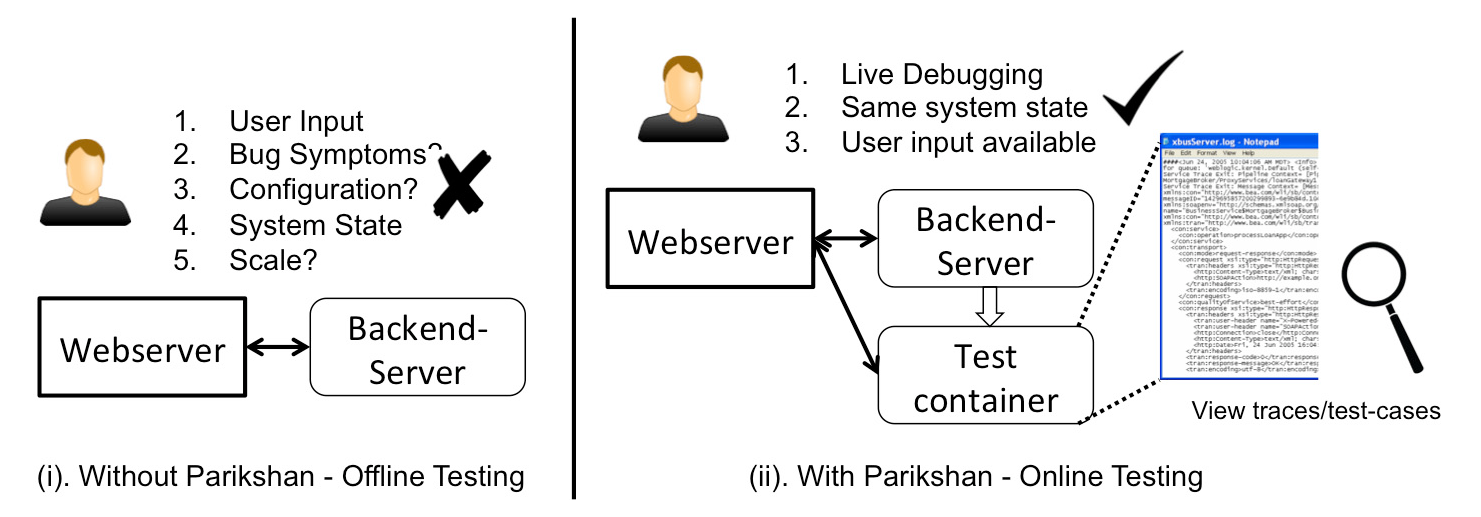
\includegraphics[width=0.7\textwidth]{figs/motivation.eps}
		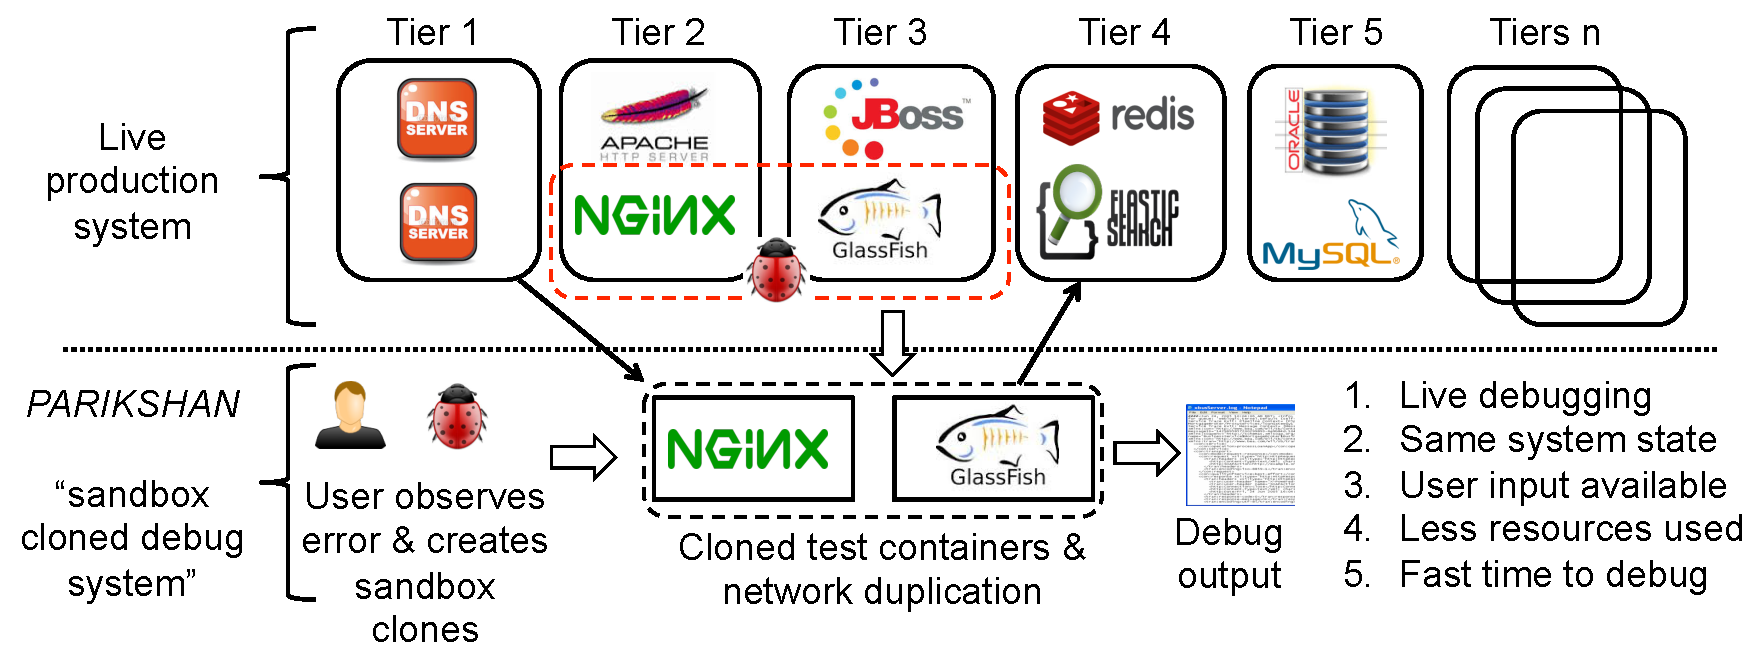
\includegraphics[width=0.9\textwidth]{figs/workflow3.pdf}
		\caption{Workflow of \parikshan in a live multi-tier production system with several interacting services. When the administrator of the system observes errors in two of it's tiers, he can create a sandboxed clone of these tiers and observe/debug them in a sandbox environment without impacting the actual production system.}
		\label{fig:motivation}
	\end{center}
\end{figure*}



\section{Background}
\label{sec:background}

In this section, we give a short description of the design of live debugging and our \parikshan framework to facilitate the exposition of the ideas in this paper. 
%A detailed explanation of the complete design of the paper can be found in ~\cite{parikshan}.

\subsection{The case for Live Debugging}
\label{sec:case}

Figure \ref{fig:motivation}, shows a high level overview of ``live debugging'' in action. 
The figure shows a live production system with multiple services. 
The system is maintained by an operator, who can observe the health of the system using light-weight monitoring, which is part of the deployed system. 
In the interest of application performance, production system monitoring is usually limited to system resource usage, application usage statistics, transaction logs, and error logs.

Let us assume that at a certain time in the execution of the system, the operator observes unusual memory usage in the glassfish application server, and some error logs being generated in the nginx webserver. 
Typically, trouble tickets are generated for such problems, and they are debugged offline.
However, the operator can now use \parikshan to fork off clones of the nginx and glassfish containers as \textbf{nginx-debug} and \textbf{glassfish-debug}.
Network duplication mechanisms ensure that the debug-containers receive the same inputs as the production, and the production containers continue to provide service without interruption.
This seperation of production and debug environments allows the operator to use dynamic instrumentation tools to do deeper diagnosis without fearing any problems in the user-facing operations.
Since the system has been cloned from the original potentially ``buggy'' production container, it will also exhibit the same memory leaks/or logical errors.
Additionally, \parikshan can focus on the ``buggy'' parts of the system, without needing to replicate the entire system in a test-cluster. This process will greatly reduce the time to bug resolution, and allow real-time bug diagnosis capability.

\subsubsection{Design Overiview}
\label{sec:design}

Our system called \parikshan, is composed of three modules: 

%\begin{itemize}
%	\item 

 \textbf{Clone Manager}: manages ``live cloning'' between the production and debug containers.
``Live Cloning'' refers to the process of copying a running virtual machine, or container from one server to another, without disconnecting any client or process running within the service.
This generates two containers, a production container which serves the actual user requests, and a debug-container which gets the same input as the production but is maintained only for debugging purposes.
The ``live'' part in the cloning process means that cloning has a very small suspend time and the service is kept active while cloning. \\

\iffalse	
	\begin{figure}[ht]
		\begin{centering}
			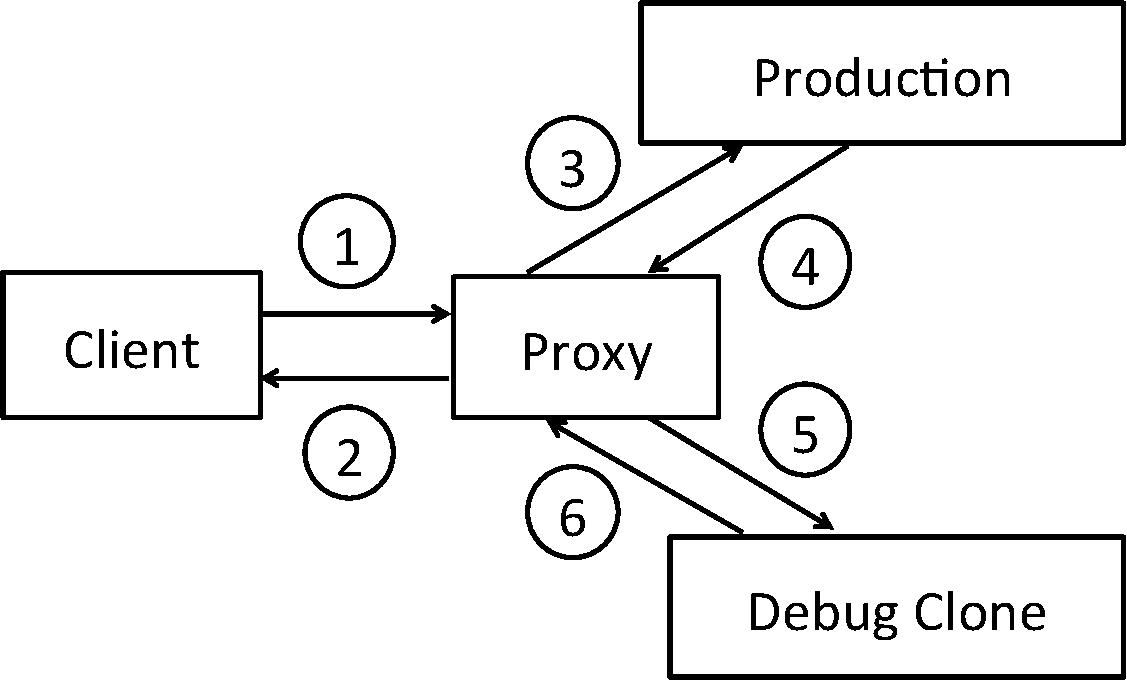
\includegraphics[width=0.4\textwidth]{figs/network_dup.pdf}
			%    \captionsetup{justification=centering}
			\caption{Description of the Network Duplicator. In \textit{synchronized} mode: Thread 1 executes steps [1,3,5], and Thread 2 executes [2,4,6] sequentially. In \textit{asynchronous} mode: Thread 1 executes steps [1,3], Thread 2 executes [2,4], Thread 3 executes [5], and Thread 4 executes [6]}
			\label{fig:duplicator}
		\end{centering}
	\end{figure}
\fi
%\item 
 \textbf{Network Duplicator}: The network duplicator manages communication from the client to both the production container and the debug container.
The basic design is based on a customized TCP level proxy, which duplicates network traffic to both these containers.
As shown in figure~\ref{fig:duplicator}, the duplicator uses an asynchronous packet forwarding model, with 4 threads for each incoming connections.
Thread T1 forwards packets from client to proxy (link 1), and from proxy to production container(link 2). It then uses a non-blocking send to foward packets to an internal pipe buffer shared between thread T1, thread T3. Thread T3, then reads from this piped buffer and sends traffic forward to the debug-container. 
Similarly Thread T2, receives packets from production container, and forwards them to the client, while thread T4, receives packets from debug container and drop them. 

The advantage of this strategy is that any slowdown in the debug-container will not impact the production container.
However, a side-effect is that if the speed of the debug-container is too slow compared to the production container, it may lead to a buffer overflow. 
We call the time taken by a connection before it overflows, it's \textbf{debugging window}.
We assume that both the production and debug containers are identical for the purposes of debugging as long as we do not have an overflow. \\

\textbf{Network Aggregator}: The network aggregator manages communication from 
	
%\end{itemize}


\section{Budget based adaptive debugging}
\label{sec:adaptive}

Here we use a statistical debugging approach which adheres to our bounded overhead.
We propose to assign to each predicate a weighted score which is associated with how frequently it should be monitored.
The sum of these weights will be equal to our bounded overhead.

In this work, we wish to establish a tradeoff between overhead of statistical debugging and the effectiveness of statistical debugging, at the same time maintaining a bounded overhead.
For instance, we can drop instrumentation of predicates which are executed more frequently to reduce the performance overhead in order to maintain our bounded overhead.
Program control and data flow inherently creates a hierarchical dependency between predicates, this can be leveraged in instrumentation to control the overhead, while at the same time provide some degree of clues to the debugger.

\subsubsection{Modeling the Target Application}

We define the program as a dynamic control-flow graph G \textless V,E \textgreater where V represent basic block entry points. 
The instrumentation granularity can be functional entries or conditionals which each should correspond to a basic block.
We call instrumentation points our predicates, where the predicate set \textless P \textgreater $\in$ \textless V \textgreater, 
i.e. each predicate can be an entry or exit point in the set of vertices's.


\subsubsection{Offline Profiling}

While not necessary, offline profiling of the target application can greatly assist in assigning weights to each predicate. 
Assuming that we have a representative input, the profile can be taken to show the time generally taken in each request, 
and every basic-block entry and exit point can be profiled to annotate time taken by each segment of the control path. 
While the processing time of each path can significantly differ depending on the input, 
we can get an approximate time taken by each section of the control flow graph for a large enough input set. 
This offline profiling helps us in assigning initial weights, and measuring the amount of slack available for each control-flow path.

\subsubsection{Assigning weight}

Weights can be defined to each predicate based on the following criteria:

\begin{itemize}
	
	\item \textbf{Importance of the predicate itself}: 
	
	The score for importance of a predicate can be defined similar to the Cooperative Bug Isolation Project (CBI) as shown in section ~\ref{sec:background-guided}. 
	
	\begin{equation}
	\label{eq:importance}
	Importance = \frac{2}{\frac{1}{Sensitivity(p)}+\frac{1}{Increase(p)}}
	\end{equation}
	
	
	\item \textbf{Slack in context of the control flow path}: 
	
	Model overall slack available based on offline instrumentation. 
	
	\item \textbf{External factors}:
	
\end{itemize}

\textit{Amortizing Predicate Calculation}: Predicate scores are updated once every n runs

\subsubsection{Online Engine}

The job of the online engine is to decide whether or not a given predicate should be sampled. 
Inputs are 


\subsubsection{Cause Isolation}
\label{sec:cause_isolation}

Cause Isolation for bugs can be done in an adaptable manner. 

We assign weight W$_{i}$ to each predicate P$_{i}$ , where the weight denotes the sampling frequency.

\begin{equation}
W_{i} = Probability\ that\ a\ predicate\ i\ is\ sampled
\end{equation}

\begin{equation}
P_{i} = Instrumentation\ Overhead\ for\ Predicate\ i
\end{equation}

\begin{equation}
\sum\limits_{i=1}^n W_{i}.P_{i} = Total\ Instrumentation\ Overhead\ Bound
\end{equation}

We have divided our approach in two halves, the first concentrates on statistical analysis for functional bugs.
Any application code can be modeled as a control flow graph 

\subsection{Motivating Example}
\label{sec:example}

We now discuss how live debugging can be used to find the cause of a bug using statistical debugging.
Take for example the code segment shown below:
\\
\par
\begin{verbbox}[\footnotesize]
	void foo {
		if(x > num and f == NULL){
			x = 0;
			*f;
		}.
	}
\end{verbbox}
\fbox{\theverbbox}\\

In this code, the \texttt{*f} is clearly an erroneous call to this pointer, and will lead to an exception.
The function \texttt{foo}, can be called by various 

\section{Related Work}
\label{sec:related}

There have been several existing approaches that look into testing applications in the wild. 
The related work can be divided in several categories:

\begin{itemize}
  
  \item \textbf{Software Debugging}
  
  In the development phase, it is common to employ debugging tools such as gnu debugger \cite{gdb}, valgrind \cite{valgrind} or just using printf statements etc.
  Several development suites\cite{eclipse, visual_studio, intel_suite} often come with inbuilt debugging capabilities, to assist developers to understand their code, and debug it as they develop new applications.
  In most cases these tools allow developers to look at the execution traces, and to insert watchpoints or breakpoints.
  In addition they allow developers to understand the context of the application by looking at variable values at different points.
  Unfortunately, this practice cannot be followed in production environments, as these tools have a high overhead.
  
  \parikshan focuses on this problem by allowing users to do live debugging of the application by cloning the production state, to produce a test-container.
  This test-container can be debugged using probes as described in \ref{sec:trigger} to give valuable insight to the developer.
  
    
  \item \textbf{Perpetual Testing}
     We are inspired by the notion of perpetual testing\cite{perpetual} which advocates that software testing should be key part of the deployment phase and not just restricted to the development phase.
  
  \item \textbf{Record and Replay}
  
  Record and Replay systems have been an area of research in the academic community for several years.
  However, almost none  
  
  \cite{altekar2009odr,dunlap2002revirt,guo2008r2, geels2007friday, laadan2010transparent}
  
  \item \textbf{A-B Testing}
  \item \textbf{Symbian Monkey}
   \item \textbf{DevOps}
\end{itemize}
  



\vspace{-1mm}
\section{Conclusion \& Future Work}
\label{sec:conclusion}

%Quick bug resolution is an important requirement for any production system maintenance effort.
%Existing techniques either add substantial overhead making them impractical in real-world systems, or are unable to capture enough trace information to localize the bug offline. 

%We presented \parikshan a framework to do live-debugging and analysis of large scale systems.
\parikshan is a novel framework that uses redundant cloud resources to debug production SOA applications in real-time.
It allows the user to diagnose and localize errors, without impacting production services.
We have shown it's applicability in  7 real-world case studies, and shown how it can be used to quickly localize the error.

In the future, we will explore: (1). Application: we aim to apply our system to real-time intrusion detection and statistical debugging.
(2). Analysis: we wish to define ``real-time'' data analysis techniques for traces and instrumentation done in \parikshan.
%We believe with streaming data analytic techniques, we can do much better than execution tracing/profiling.
(3). We plan to reduce the suspend time of live cloning, by utilizing several recent works in live migration.
We also tested \parikshan on Google's Cloud Infrastructure (Google Compute~\cite{gcompute}) and plan to use this for future work. 
%Running a clone in the same machine as the production container opens several venues such as copy-on-write migration, and asynchronous container syncing etc.

An extended version of the paper is present in CUCS Tech Reports~\cite{parikshanTR,parikshanQueue}, details about the project, and source code is available on github~\cite{github}. 
Kaiser is funded in part by NSF CCF-1302269 and CCF-1161079.
%comment{
%We would like to acknowledge Qiang Xu, Abhishek Sharma, and Pallavi Joshi for their insight and feedback in designing \parikshan, and in the evaluation of this technology.
%The authors are affiliated with NEC Labs, Princeton, Google Inc, and Columbia University. 



\bibliographystyle{abbrv}
\bibliography{guided}  % sigproc.bib is the name of the Bibliography in this case
% You must have a proper ".bib" file
%  and remember to run:
% latex bibtex latex latex
% to resolve all references
\end{document}
